\documentclass{article}
%\VignetteIndexEntry{traitr}
%\VignettePackage{traitr}

\usepackage{fancyhdr}
\lhead{The \texttt{traitr} package}
\rhead{Page \thepage}
\renewcommand{\headrulewidth}{0.4pt}
\pagestyle{fancy}

\usepackage{geometry}
\usepackage{mathptmx} 
\usepackage[pdftex]{graphicx}           % for graphics files
\usepackage{relsize}            % for relative size fonts
\usepackage{amsmath}            % for amslatex stuff
\usepackage{amsfonts}           % for amsfonts
\usepackage{url}                % for \url,
\usepackage{booktabs}
\usepackage{fancyvrb}

\usepackage[T1]{fontenc}
%\usepackage[adobe-utopia]{mathdesign}
%\usepackage{aurical}

\renewcommand{\encodingdefault}{T1}
\usepackage[sc]{mathpazo}
\linespread{1.05}         % Palatino needs more leading (space between lines)


\newcommand{\R}{\textsf{R}}
\newcommand{\code}[1]{\texttt{#1}} % code
\newcommand{\command}[1]{\code{#1}} % name of command
\newcommand{\function}[1]{\code{#1}} % name of function
\newcommand{\constructor}[1]{\function{#1}\index{#1}}
\newcommand{\args}[1]{\code{#1}} % name of argument only
\newcommand{\class}[1]{\code{#1}}  % a class
\newcommand{\generic}[1]{\code{#1}} % name of generic method -- no
\newcommand{\meth}[1]{\generic{#1}}     % single arg, no class
\newcommand{\property}[1]{\code{#1}}     % single arg, no class
\newcommand{\object}[1]{\code{#1}}

\newcommand{\qcode}[1]{\code{"#1"}} % quoted code 

\newcommand{\defn}[1]{\textit{#1}\index{\textit{#1}}}   % add in index


\newcommand{\argument}[2]{\args{#1}\index{#2|\texttt{#1}}} % name of an argument, plus
                                % function for index
\newcommand{\subcommand}[2]{\textit{#2} \args{#1}\index{#2|\code{#1}}} % name of an tk subcommand plus
                                % function for index
\newcommand{\subcommanda}[3]{\subcommand{#1}{#2} \textit{#3} }
\newcommand{\option}[2]{\args{#1}\index{#2|\code{#1}}} % name of an option plus constructor

\newcommand{\method}[1]{\meth{#1}}%\index{#2|\code{#1}}} % name of method with
                                % class for index

\newcommand{\signal}[1]{\code{#1}} % name of signal
\newcommand{\dfn}[1]{\textit{#1}} % definition
\newcommand{\dfnref}[1]{\textit{#1}} % refer to a definition
\newcommand{\env}[1]{\texttt{#1}} % environment setting
\newcommand{\file}[1]{\texttt{#1}}
\newcommand{\kbd}[1]{\textmd{#1}}
\newcommand{\pkg}[1]{\texttt{#1}}
\newcommand{\opt}[1]{\texttt{#1}} % R option
\newcommand{\acronym}[1]{\texttt{#1}}

%% Begin here
\usepackage{/Users/Verzani/R/R.framework/Resources/share/texmf/Sweave}
\begin{document}
\thispagestyle{empty}

\thispagestyle{empty}
\bibliographystyle{plainnat}


%% Introduction
\title{The traitr package}
\author{John Verzani\\\texttt{verzani at math dot csi dot cuny dot edu}}
\maketitle
\begin{abstract}
  This vignette describes the \pkg{traitr} package. This package
  provides an interface to GUI design within R in the spirit of the
  \code{Traits UI} python module. The basic idea
  is that the user specifies the type of data that is desired, and the
  package gives a reasonable GUI to edit that data.
 \end{abstract}
 
\section{Five-minute, or so, introduction}
\label{sec:five-minute-intr}

The \pkg{traitr} package is intended to provide a natural, relatively
easy means to produce GUIs for underlying functions. The design was inspired by
the \code{Traits UI} python module
(\url{http://code.enthought.com/projects/traits}), although the
implementation is not nearly as feature rich as that.

The \code{Traits UI} interface uses the model-view-controller design
pattern. The main idea is that a user specifies a model consisting of
possibly many properties, each holding data of a certain type. Each
property we call an item. A view of the model is specified by
indicating which items are to be shown along with a layout. The items
themselves know how to present themselves graphically so that the user
can interact, or edit, the values. One then ties the model and view
together by specifying some common methods (a controller).

This provides a simple map between a function with arguments
(whose values are of a certain type) and a GUI to edit these values,
which makes the writing of basic GUI dialogs for R functions very
straightforward -- no GUI
programming is needed.~\footnote{This vignette documents
  version 0.9 of the package.}

The \pkg{traitr} package uses \pkg{gWidgets} to provide a link to a
graphical toolkit. At this point it works with \pkg{gWidgetsRGtk2} and
\pkg{gWidgetsQt}, but there are issues with \pkg{gWidgetstcltk}.

There are a few means available now within \R{} to have GUIs automatically written
for you such as \pkg{fgui} and the \pkg{ggenericwidget} function in
\pkg{gwidgets}. The basic idea employed is an inspection of a function's arguments to
determine the type of data expected and the a determination of the
appropriate widget for editing that
type. This package provides \constructor{dialogMaker} to do so, but
also make it easy for the user to just
specify the data type for the arguments to make a GUI. 

The basic unit in \pkg{traitr} is an item, which is an object that
knows what type of value it should hold and how to represent that
value in a GUI. Since the programmer knows the type of value they
want, this isn't difficult to provide, yet the GUI creation aspect is
mostly hidden from sight -- unless the programmer wishes to change the
defaults. The GUI for an item is referred to as an editor, as in most
cases, the primary usage is to display the underlying value for
editing.


At this point, there are a few basic type of items listed in
Table~\ref{tab:item-constructors}. Adding more is on the TODO list.
\\

\subsection{A first example}
\label{sec:first-example}


To begin with \pkg{traitr}, we load the package and specify a
\pkg{gWidgets} implementation. 

\begin{Schunk}
\begin{Sinput}
 require(traitr)
 require(gWidgets)
 options(guiToolkit="RGtk2")
\end{Sinput}
\end{Schunk}

An item constructor is called with a default value and possibly many
other values. Items may be combined into ``item groups'' or
``dialogs,'' the latter being an item group with a window and a set of
buttons. 

To see how a simple GUI can be made, here we construct a GUI to
collect a number and string:
\begin{Schunk}
\begin{Sinput}
 dlg <- aDialog(items=list(
                  number=numericItem(0),
                  string=stringItem("")
                  )
                )
 dlg$make_gui()                          # method call using $ notation.
\end{Sinput}
\end{Schunk}

\begin{figure}
  \centering
  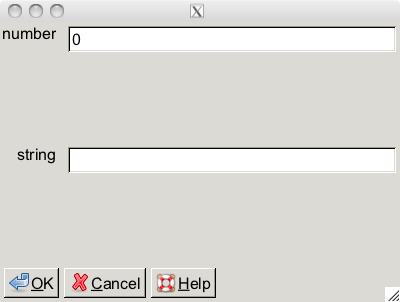
\includegraphics[width=.6\textwidth]{basic-gui}
  \caption{Basic  interface with two items, a number and string.}
  \label{fig:basic-gui}
\end{figure}

The \constructor{aDialog} constructor returns a \pkg{proto} object for
which there are many methods defined, but just a few that are
necessary to know. In this instance, we use the dialog's
\meth{make\_gui} method to create the GUI. To see other documented
methods and properties of the \pkg{proto} objects produced, call their
\meth{show\_help} method.~\footnote{The \pkg{proto} package extends
  R's environments to implement a prototype programming style. To call
  a function, we use the \code{\$} notation to reference the
  function. Unlike storing a function in a regular environment, this
  function call passes back into the function, as the first argument,
  a reference to the \pkg{proto} object. As such, the function
  signature would be something like \code{(self, arg1, arg2)}, where
  self is used here for familiarity with javascript (another prototype
  language). However, it is traditional to use \object{.} as this
  variable instead of \object{self}, so we use this in the code, as
  needed.} That is, this command will produce a web page with the
information for the \code{dlg} instance: \code{dlg\$show\_help()}.

The default dialog GUI has three buttons, an OK button (which when clicked
prints out the values in the GUI), a Cancel button to dismiss the
dialog and a Help button to call up a simple help string, which in
this example is not implemented. To change the buttons, one assigns
the names to the \property{buttons} property of the dialog. The values
``Undo'' and ``Redo'' will implement the undo/redo pattern for the
underlying model.

To override the default behaviours or to assign actions to other
buttons, one defines methods for the dialog object using a certain
naming convention. For the dialog buttons, if one defines a function
(\meth{buttonname\_handler}), then this will be called when the button
``buttonname'' is clicked. For example, to make the dialog do
something else, we have:
\begin{Schunk}
\begin{Sinput}
 dlg <- aDialog(items=list(
                  number=numericItem(0),
                  string=stringItem("")
                  ),
                OK_handler=function(.) { # . is reference to dlg object
                  values <- .$to_R()
                  f <- function(number,string) 
                    cat("number is", number, "string is", string, "\n")
                  do.call(f, values)
                }
                )
 dlg$make_gui()
\end{Sinput}
\end{Schunk}

The function \meth{OK\_handler} becomes a method of the \pkg{proto}
object, so its lone argument \object{.} passes into the function body the
\pkg{proto} object. (These objects are environments, so the usual pass
by copy is not used, rather this is the same object.) Its method \meth{to\_R} returns a named list of
the values stored for each item in the dialog -- which is convenient
for \code{do.call} --  and this handler simply
echoes them back in a friendly manner. Individual properties in the
dialog can be accessed through ``getters.'' These follow the naming
convention \code{get\_PROPERTYNAME}, as in
\begin{Schunk}
\begin{Sinput}
 dlg$get_number()
\end{Sinput}
\begin{Soutput}
[1] 0
\end{Soutput}
\end{Schunk}
(The \code{number} is the name assigned to the item. In this case --
since it is not specified in an argument -- it
gets it from the named component of the list where the item is defined.)

To make a less trivial dialog we just need to have more complicated
functions. What follows is a dialog~(Figure~\ref{fig:t-test-1}) for computing a $t$-test when the
values are summarized. First a function to compute the $p$-value.
%% basic -- t.test
\begin{Schunk}
\begin{Sinput}
 basic.t.test <- function(mean, mu, sd, alternative=c("two.sided","less","greater"),
                          n, ...) {
   alternative <- match.arg(alternative)
   obs <- (mean - mu)/(sd/sqrt(n))
   switch(alternative,
          "greater" = 1 - pt(obs, df=n-1),
          "less" = pt(obs, df=n-1),
          2*(1 - pt(abs(obs), df=n-1))
          )
 }
\end{Sinput}
\end{Schunk}
Our dialog setup is similar, but we have more variables that need
their type specified:
\begin{Schunk}
\begin{Sinput}
 dlg <- aDialog(items=list(
                  mean=numericItem(0),
                  sd=numericItem(1),
                  n=numericItem(5),
                  mu=numericItem(0),
                  alternative=choiceItem("two.sided", values=c("two.sided","less","greater")),
                  output=stringItem("", label="p.value")
                  ),
                title="A basic t-test interface",
                help_string="Enter in summarized values then click OK to get the p-value",
                OK_handler=function(.) {
                  lst <- .$to_R()
                  lst$output <- NULL     # not really needed, ignored by function 
                  out <- do.call("basic.t.test", lst)
                  .$set_output(out)
                }
                )
 dlg$make_gui()
\end{Sinput}
\end{Schunk}
 
\begin{figure}
  \centering
  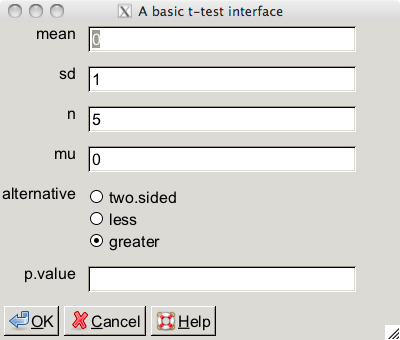
\includegraphics[width=.6\textwidth]{t-test-1}
  \caption{Basic $t$-test interface}
  \label{fig:t-test-1}
\end{figure}

Here we used the \constructor{choiceItem} to provide a choice to the
user. As well, we added values for the title and  help string. The
handler has the method call \meth{set\_output} to set the value to
show in the output widget. When a dialog is created, both ``\code{get}'' and ``\code{set}''
methods are created for each item specified, where \code{output}
matches the \code{name} property of the item (which is specified
through the named list passed to \code{items}).


\subsection{Views}
\label{sec:views}

\begin{figure}
  \centering
  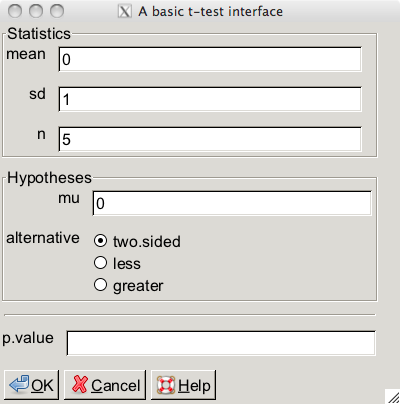
\includegraphics[width=.6\textwidth]{t-test-2}
  \caption{The $t$-test interface using an alternate view that
    separates off the statistics from the hypotheses.}
  \label{fig:t-test-2}
\end{figure}


The default GUI layout uses a 2-column table to organize the
items. To modify this, one creates an alternate view or layout for the
items. There are a few view constructors, similar to the containers in
\pkg{gWidgets}. Table~\ref{tab:view-constructors} lists them.


The basic layout is equivalent to:
\begin{Schunk}
\begin{Sinput}
 view <- aContainer("mean","sd","n","mu","alternative","output")
\end{Sinput}
\end{Schunk}
The \constructor{aContainer} constructor simply lays out its child components
using a two-column table, one for the label and one for the widget
representing the item.
The items are specified by name. (The name can be explicitly set when
the item is constructed, e.g. \code{numericItem(1, name="x")} or, as
in the example, found from using a named list to define the items.)

To make a more complicated layout, we nest the containers. Here is how
one can separate out the computed values from the hypotheses using frames:
\begin{Schunk}
\begin{Sinput}
 view <- aContainer(aFrame("mean","sd","n", label="Statistics"),
                    aFrame("mu", "alternative", label="Hypotheses"),
                    "output")
\end{Sinput}
\end{Schunk}

However, this view will not align values, as the \constructor{aFrame}
container is just a box container. Instead we add in another
level with \constructor{aContainer} (Figure~\ref{fig:t-test-2}):
\begin{Schunk}
\begin{Sinput}
 view <- aContainer(aFrame(aContainer("mean","sd","n"), label="Statistics"),
                    aFrame(aContainer("mu","alternative"),label="Hypotheses"),
                    separatorItem(),
                    "output")
\end{Sinput}
\end{Schunk}
To see this in action, to save typing, we use the \meth{instance} method, which for this purpose
simply copies the
dialog object. Then to specify a view different than the default, we
use the \args{gui\_layout} argument of the \meth{make\_gui} method:
\begin{Schunk}
\begin{Sinput}
 dlg1 <- dlg$instance() ## instead of copying the definition above.
 dlg1$make_gui(gui_layout=view)
\end{Sinput}
\end{Schunk}


\subsection{Validation}
\label{sec:validation}

Items use the model-view-controller design pattern, with a transport
phase from view to model that allows for inspection of values. As
such, we can check for valid input when assigning from the view to the
model.~\footnote{Although we allow invalid input for technical
  reasons. It isn't until the call to \meth{to\_R} that an issue will
  arise.} When an item has invalid input, some signal is specified. To
see it, try typing in a non-numeric value in where a number is
expected.

To see how to specify our own validation function,~\footnote{Validation
  is done for the main value stored in an item. For more complicated
  items using more than one main property, one can defind
  \meth{validate\_PROPERTYNAME} methods.  } we first write the
function, then add it to the item. For the standard deviation, we
shouldn't be able to specify non-positive standard deviations. A
function to check this would be:
\begin{Schunk}
\begin{Sinput}
 positive_value <- function(., rawvalue) {
   value <- as.numeric(rawvalue)
   if(!value > 0)
     stop("value is not positive")
   value
 }
\end{Sinput}
\end{Schunk}

The \object{.} argument is the item instance (not the dialog, say) and
the argument \args{rawvalue} comes from the widget. (In this case a
string, so we coerce the value before testing.) The validation
functions should throw an error with a message if not valid. (The item
itself has a \meth{coerce\_with} method to carry out the proper coercion.)

To add to a numeric item, we assign to its \meth{validate}
method:~\footnote{Here we see the ease of using the \pkg{proto}
  package, but it is also a burden. It is quite possible to assign to a
``private'' method, thereby having very unintended side effects that
can be hard to debug.}
\begin{Schunk}
\begin{Sinput}
 sd <- numericItem(1, name="sd")
 sd$validate <- positive_value
\end{Sinput}
\end{Schunk}


To do this for our dialog object, we can grab the item from the
dialog, then specify its validation method:
\begin{Schunk}
\begin{Sinput}
 sd <- dlg$get_item_by_name("sd")         # lookup and return item by name
 sd$validate <- positive_value            # assigns method to item
 dlg1 <- dlg$instance()
 dlg1$make_gui(gui_layout=view)
\end{Sinput}
\end{Schunk}


\subsection{Conditional layout}
\label{sec:conditional-layout}
Parts of a view can be enabled conditioned on other parts of the
GUI. In this example we make a GUI~(Figure \ref{fig:t-test-enabled}) for a one or two-sample
$t$-test. As some options (such as \args{paired}) only make sense when
two samples are specified, we enable those only when a possible value
for \code{y} is specified. In the \code{x} and \code{y} items, the
argument \code{eval=TRUE} is specified, which causes the specified
value to be parsed and evaluated in the global environment. This allows the
user to specify a variable name or \R\/ expression for the variable,
and not just a number. 

\begin{Schunk}
\begin{Sinput}
 dlg <- aDialog(items=list(
                  x = numericItem(NA, eval=TRUE),
                  y = numericItem(NA, eval=TRUE),
                  alternative=choiceItem("two.sided", 
                    values=c("two.sided", "less", "greater")),
                  mu = numericItem(0),
                  paired=trueFalseItem(FALSE),
                  var.equal=trueFalseItem(FALSE)
                  ),
                title="GUI with some parts disabled"
                )
 view <- aContainer("x",
                    aContext("y", context=dlg,
                             enabled_when=function(.) { # y depends on x
                               ## . here is the context value, not the container object
                               val <- .$to_R()$x
                               !is.null(val) && !is.na(val)  && (nchar(val) > 0)
                             }),
                    "alternative",
                    "mu",
                    aContainer("paired","var.equal", context=dlg,
                               enabled_when=function(.) {
                                 val <- .$to_R()$y
                                 !is.null(val) && !is.na(val) &&  (nchar(.$get_y()) > 0)
                               })
                    )
 dlg$make_gui(gui_layout=view)
\end{Sinput}
\end{Schunk}
The \constructor{aContext} container is used to specify optional arguments to
the view, but does not do any layout. In this case, the \code{y} value
is conditioned on the value specified for \code{x}. The \args{context}
argument specifies a dialog (or item group) where the variable is to
be looked up.


\begin{figure}
  \centering
  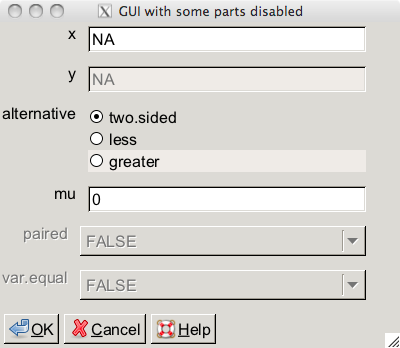
\includegraphics[width=.6\textwidth]{t-test-enabled}
  \caption{A $t$-test interface with some items having sensitivity
    depending on values of other items.}
  \label{fig:t-test-enabled}
\end{figure}



\subsection{Why wait?}
\label{sec:why-wait}

The basic dialog calls a function when the OK button is clicked. 
Making a more interactive GUI, say to update when a value is changed,
can be done by creating a method \meth{model\_value\_changed}. For
example, here is a GUI~(Figure \ref{fig:why-wait}) to draw a graph for a random sample of size $n$.
\begin{Schunk}
\begin{Sinput}
 drawGraph <- function(n,..) hist(rnorm(n))
 dlg <- aDialog(items=list(
                  n=rangeItem(10, from=1, to=100, by=1),
                  graph=graphicDeviceItem()
                  ),
                title="Draw a graph",
                help_string="Adjust slider or click OK to produce a new graph",
                model_value_changed=function(.) {
                  l <- .$to_R()
                  l$graph <- NULL        # not really necessary
                  do.call("drawGraph", l)
                },
                OK_handler=function(.) do.call("drawGraph",.$to_R())
                )
 dlg$make_gui()
\end{Sinput}
\end{Schunk}


\begin{figure}
  \centering
  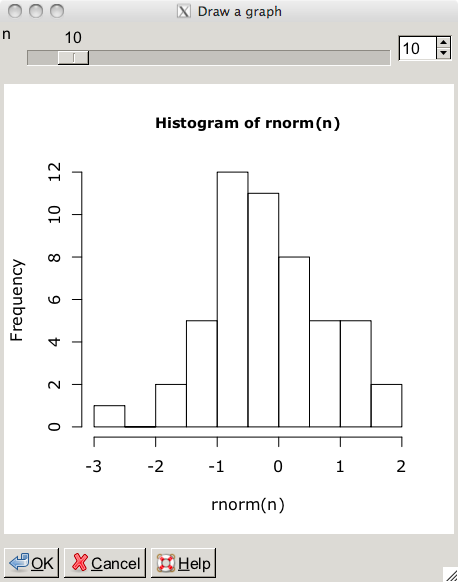
\includegraphics[width=.6\textwidth]{why-wait}
  \caption{GUI where slider movement updates the graphic.}
  \label{fig:why-wait}
\end{figure}

The dialog is a model that observes itself for changes. When such a
change occurs, methods matching a certain naming convention are
called. The \code{model\_value\_changed} method, if present, is always
called when any property is changed.

%%%%%%%%%%%%%%%%%%%%%%%%%%%%%%%%%%%%%%%%%%%%%%%%%%
%% Items

\section{Items}
\label{sec:items}
The basic object in \pkg{traitr} is an item. An item includes a model
to keep track of its value(s), an editor (the view) to create a GUI to edit the
value(s) and a controller to link the two. In addition, items may
include methods for validation of its values. Following the design of
\code{Traits UI}, items allow the programmer to focus on the type of
value, not the GUI presentation of the value.

Items are constructed through one of the item
constructors. Table~\ref{tab:item-constructors} lists the currently
available ones. The constructors have some common arguments:
\args{value} to specify the initial value of the item; \args{name}
to specify the unique name for the item within a dialog (this can also
be specified through a named list); \args{label} for a text label to
identify the argument (defaults to \args{name}); \args{tooltip} to
specify a tooltip for the widget, should it provide one; \args{attr}
to pass arguments to the \pkg{gWidgets} constructor underlying the
editor; \args{model} to specify a model for the item (models can be
shared, or a new one will be created); and \args{editor} to specify a
different editor.

In addition to these, each item has some item-specific arguments. For
example, \constructor{numericItem} and \constructor{integerItem} have an argument
\args{eval\_first} which if set to \code{TRUE} will force the value
from the editor to be evaluated within the global environment as a string.


\begin{table}
\centering
\label{tab:item-constructors}
\caption{Table of item constructors.}
\begin{tabular}{@{}lp{0.7\textwidth}@{}}
\toprule

Constructor&Description\\
\midrule
stringItem&For holding strings\\numericItem&For numbers\\integerItem&For integers\\expressionItem&For R expressions\\trueFalseItem&For Boolean values\\choiceItem&For choosing one or more values from a list of possible values\\rangeItem&To select a value from a range of values\\buttonItem&For adding a button\\labelItem&For adding a label\\dateItem&For editing a calendar date.\\separatorItem&To add a visual separator\\dataframeItem&To select a data frame\\variableSelectorItem&To select a variable from a data frame\\graphicDeviceItem&(RGtk2 only) To embed a graphic device\\formulaItem&For formula specification (to be written)\\dfeditItem&To edit a data set (to be written)\\itemList&An item that stores a list of other items (or itemgroups)
\\ \bottomrule
\end{tabular}
\end{table}
The \constructor{choiceItem} provides a means to choose a value for a
specified list of values. The editor may use a radio button group, a
checkbox group, a combobox or a table widget to present the choice
depending on the size of the list of values and whether multiple
selection is possible. The constructor has two arguments, \args{value}
to specify the initially chosen value and \args{values} to specify the
list to choose from.  The former can be specified by value (the
default) or by index (if \code{by\_index=FALSE} is give).  The latter
may be a vector or data frame.

The \constructor{dataframeItem} constructor provides a means to select
a data frame. The \constructor{variableSelectorItem} constructor
requires such an object to be passed to it, in order for it to have a
context to find names in. For example

\begin{Schunk}
\begin{Sinput}
 dfi <- dataframeItem(value=".GlobalEnv", name="dfi", 
                      editor_style="compact") # alternative editor style
 dlg <- aDialog(items=list(
                  dfi,
                  vsi=variableSelectorItem("", multiple=FALSE, dataframeItem=dfi, 
                    attr=list(size=c(200,200)))
                  ))
 dlg$make_gui()
\end{Sinput}
\end{Schunk}

The \constructor{itemList} constructor is used to create a list of items or item
groups. See~\ref{sec:codeitemlist-item} for examples.


% http://yuml.me/diagram/scruffy/class/[Model] -> [Item|get/set_editor;visible_when;enabled_when; validate; get/set_model| show_label; tooltip]

\begin{figure}
  \centering
  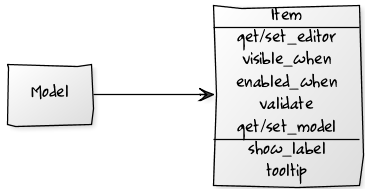
\includegraphics[]{uml-items}
  \caption{Standard methods and properties for an Item. (All
      UML diagrams come from \texttt{http://yuml.me/})}
  \label{fig:uml-items}
\end{figure}

\subsection{Item groups}
\label{sec:item-groups}


An \object{ItemGroup} is used by \constructor{aDialog} to combine more than one
item into a unit which acts as the model for the GUI. The \constructor{anItemGroup} constructor is similar to
that for a dialog, but is used if one wants to embed the resulting GUI
into some \pkg{gWidgets} container without the buttons, menubar, and
toolbar options.

Item groups implement the model interface, described in the next section.

Item groups can allow for resuse of parts of a GUI. In this example, we
see how we can separate some pieces out that are common to both a
$t$-test and a Wilcox test call:
\begin{Schunk}
\begin{Sinput}
 hyps <- anItemGroup(items=list(
                       mu=numericItem(0), 
                       alternative=choiceItem("two.sided", c("two.sided","less","greater"))
                       ),
                     gui_layout=aFrame("mu","alternative", label="Hypotheses")
                     )
 ttestDialog <- aDialog(items=list(
                          x=numericItem(NA, eval=TRUE),
                          y=numericItem(NA, eval=TRUE),
                          hyps$instance()
                          ),
                        OK_handler=function(.) {
                          do.call("t.test",.$to_R())
                        }
                        )
 wilcoxDialog <- aDialog(items=list(
                           x=numericItem(NA, eval=TRUE),
                           y=numericItem(NA, eval=TRUE),
                           hyps$instance()
                           ),
                         OK_handler=function(.) {
                           do.call("wilcox.test", .$to_R())
                         }
                         )
 ttestDialog$make_gui()
 wilcoxDialog$make_gui()                 # shares alt info!
\end{Sinput}
\end{Schunk}

The use of \meth{instance} ties the models together, but allows for
multiple views. This may not be desirable. If two independent
realizations are desired, then creating a factory (a function) to
produce new instances of \code{hyps} would be suggested.

% http://yuml.me/diagram/scruffy/class/[Model] ->
% [ItemGroup|get_items;get_item_by_name;to_R;to_string;make_gui;
% visible; enabled; get/set_model;instance;update_ui|items]

\begin{figure}
  \centering
  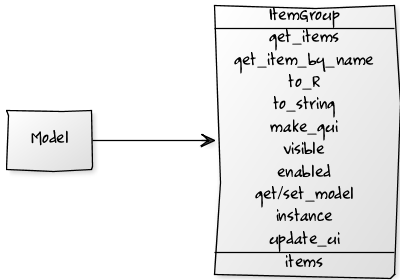
\includegraphics[]{uml-itemgroup}
  \caption{Standard methods and properties for an item group.}
  \label{fig:uml-itemgroup}
\end{figure}
  

%%%%%%%%%%%%%%%%%%%%%%%%%%%%%%%%%%%%%%%%%%%%%%%%%%
%% Models
\section{Models}
\label{sec:models}

Each item (and item group) implements a model interface. The
underlying items uses the model-view-controller design pattern. A
model is a object with a means to store and access properties and a mechanism to
notify observers when these properties have changed.


\subsection{Getters/Setters}
\label{sec:getterssetters}

Each model property has \meth{get} and \meth{set} methods to interact
with the value stored in the model. For an item with a given name,
say \code{x}, there are always methods \meth{get\_x} to get the value
and \meth{set\_x} to set the value. The get method returns a raw
value, unlike the method \meth{to\_R} which returns a value after
coercion to the appropriate type. For example:
\begin{Schunk}
\begin{Sinput}
 i <- numericItem(0, name="item1")
 i$get_item1()
\end{Sinput}
\begin{Soutput}
[1] 0
\end{Soutput}
\begin{Sinput}
 i$set_item1(3)
 i$get_item1()
\end{Sinput}
\begin{Soutput}
[1] 3
\end{Soutput}
\begin{Sinput}
 try(i$set_item1("c(1,2,3)"))            # fails validation, still stored in model
\end{Sinput}
\begin{Soutput}
Not a valid value: Error in function (., value)  : 
  (converted from warning) NAs introduced by coercion
\end{Soutput}
\begin{Sinput}
 i$get_item1()
\end{Sinput}
\begin{Soutput}
[1] "c(1,2,3)"
\end{Soutput}
\end{Schunk}

Where as, we can have the value run through \code{eval} to have:
\begin{Schunk}
\begin{Sinput}
 i <- numericItem(0, name="item2", eval=TRUE)
 i$set_item2("c(1,2,3)")                 # now okay
 i$get_item2()
\end{Sinput}
\begin{Soutput}
[1] "c(1,2,3)"
\end{Soutput}
\begin{Sinput}
 i$to_R()                                # coerced
\end{Sinput}
\begin{Soutput}
$item2
[1] 1 2 3
\end{Soutput}
\end{Schunk}

Item groups and dialogs also implement these methods, as they act as
models with several properties:
\begin{Schunk}
\begin{Sinput}
 dlg <- aDialog(items=list(
                  x=numericItem(0),
                  y=stringItem("a")
                  ))
 dlg$get_x()
\end{Sinput}
\begin{Soutput}
[1] 0
\end{Soutput}
\begin{Sinput}
 dlg$set_y("some string")
 dlg$get_y()
\end{Sinput}
\begin{Soutput}
[1] "some string"
\end{Soutput}
\end{Schunk}


\subsubsection{Getting/Setting other values in an item}
\label{sec:gett-other-valu}

If an item in an item group has more than one main property, the main
getter/setter pairs created from each item name do not suffice. For
example, the choice item has a main property for setting the value,
but another property to store the values to choose from. To access a
secondary property, we first extract the item by name with the
\meth{get\_item\_by\_name} method of item groups, and then use the item's
getter/setter values. For example:
\begin{Schunk}
\begin{Sinput}
 ig <- anItemGroup(items=list(
                   x=numericItem(1),
                   y=choiceItem("a", values=letters[1:5])
                     )
                   )
 ig$get_y()
\end{Sinput}
\begin{Soutput}
[1] "a"
\end{Soutput}
\begin{Sinput}
 i <- ig$get_item_by_name("y")
 i$get_y()                               # same as above
\end{Sinput}
\begin{Soutput}
[1] "a"
\end{Soutput}
\begin{Sinput}
 i$get_values()                          # get values
\end{Sinput}
\begin{Soutput}
[1] "a" "b" "c" "d" "e"
\end{Soutput}
\begin{Sinput}
 i$set_values(letters)                   # to set values
\end{Sinput}
\end{Schunk}


\subsection{Observers}
\label{sec:observers-1}

Models implement the observer pattern. An observer is notified
whenever a specific model property changes or if any of the model's properties changes. To do so,
the observer (which is a model instance like an item, item group, or
dialog; or a controller) would have methods
\meth{model\_value\_changed} which is called whenever any property is
changed or \meth{property\_NAME\_value\_changed} which is called when
a given property is changed. 

To add an observer to a model, the \meth{add\_observer} method is
used, whereas \meth{remove\_observer} is provided to remove the observer.
This example defines two dialogs, the second with a suitably named
method and then has the second observer change in the first.
\begin{Schunk}
\begin{Sinput}
 dlg <- aDialog(items=list(
                  x=numericItem(0),
                  y=numericItem(0)
                  )
                )
 dlg1 <- aDialog(items=list(
                   a=numericItem(0)
                   ),
                 property_x_value_changed=function(., value, old_value) {
                   .$set_a(.$get_a() + value) # add value to a (assumes numeric)
                 }
                 )
 dlg$add_observer(dlg1)
 dlg1$get_a()
\end{Sinput}
\begin{Soutput}
[1] 0
\end{Soutput}
\begin{Sinput}
 dlg$set_x(10)
 dlg1$get_a()                            # updated by x
\end{Sinput}
\begin{Soutput}
[1] 10
\end{Soutput}
\end{Schunk}

A dialog listens to itself, which allows the change of one property
to update another. This example shows how the image is updated whenever
the file is changed.

\begin{Schunk}
\begin{Sinput}
 dlg <- aDialog(items=list(
                  f=fileItem(""),
                  i=imageItem("",attr=list(size=c(480,480)))
                  ),
                property_f_value_changed=function(., value, old_value) {
                  .$set_i(value)
                },
                buttons="Cancel")
 dlg$make_gui()
\end{Sinput}
\end{Schunk}

The \meth{model\_value\_changed} method has previously been
illustrated. This method is called whenever any value is changed in
the model.



\subsection{Sharing a model}
\label{sec:sharing-model}
An item can share a model with another item. This allows for
synchronization of values in a GUI. There are several means to do
this: specifying the model at construction, calling the
\meth{set\_model} method, or calling the \meth{instance} method. For example,
\begin{Schunk}
\begin{Sinput}
 i <- numericItem(0, name="x")
 j <- numericItem(1, name="x")
 j$get_x()
\end{Sinput}
\begin{Soutput}
[1] 1
\end{Soutput}
\begin{Sinput}
 j$set_model(i)
 j$get_x()
\end{Sinput}
\begin{Soutput}
[1] 0
\end{Soutput}
\begin{Sinput}
 i$set_x(10)
 j$get_x()
\end{Sinput}
\begin{Soutput}
[1] 10
\end{Soutput}
\end{Schunk}

The \meth{instance} method also creates a new item with a shared
model, or as seen, a new dialog with shared models. There can only be
one GUI for an instance of an item, but different instances can have
GUIs, allowing multiple views for the same model.



%% http://yuml.me/diagram/scruffy/class/[Model|get/set_PROPERTYNAME;add/remove_observer;
%% notify_observers;getattr; setattr|PROPERTIES ]

\begin{figure}
  \centering
  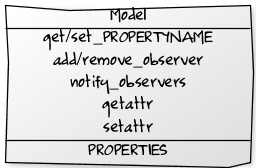
\includegraphics[]{uml-model}
  \caption{Standard methods and properties for a model.}
  \label{fig:uml-model}
\end{figure}



\section{Dialogs}
\label{sec:dialogs}

Dialogs and item groups combine several items into a model, with different
properties. In addition to the getter/setter methods, there is the
useful \meth{get\_item\_by\_name} to retrieve a given item, and
\meth{to\_R} method to get the values as a named list.

A dialog is an item group which creates its own top-level window. As
such, dialogs have options for decorating the window: e.g., to add
menubars, toolbars, and statusbars etc.
We've seen how specifying the title and help string at construction is
done through the argument \args{title} and \args{help\_string}.

The top-level container is constructed by a call to the
\meth{make\_gui} method. To close the GUI programmatically, the
\meth{close\_gui} method is available.

\subsection{Menubars, toolbars, statusbars}
\label{sec:menub-toolb-stat}

Menu bars and toolbars are specified using \pkg{gWidgets}
objects. Basically, a list of \constructor{gaction} objects (of
\pkg{gWidgets}) are specified to
the dialog properties \args{menu\_list} and \args{toolbar\_list}. 

\begin{Schunk}
\begin{Sinput}
 mb_l <- list(File=list(
                New=gaction("new", icon="new", handler=function(h,...) print("New")),
                Quit=gaction("quit", icon="quit", handler=function(h,...) dlg$close_gui())
                ))
 tb_l <- list(Quit=gaction("quit", icon="quit", handler=function(h,...) dlg$close_gui()))
 dlg <- aDialog(items=list(x=stringItem("some value")),
                menu_list=mb_l,
                toolbar_list=tb_l,
                title="Dialog with menu and toolbar")
 dlg$make_gui()
\end{Sinput}
\end{Schunk}
    

A status bar is created if the value of the
\property{status\_text} property is non \code{NULL}, say \code{""}, when \meth{make\_gui}
is called. If there is a status bar, the method
\meth{update\_status\_text} is provided.

\subsection{Buttons}
\label{sec:buttons}

Dialogs have a default set of buttons: OK, Cancel and Help. When
clicked these call the methods \meth{OK\_handler},
\meth{Cancel\_handler} and \meth{Help\_Handler}. As well, buttons
named Undo and Redo have default handlers if specified. Likely, only
\meth{OK\_handler} will need to be overridden. An example was
previously given.

To specify other buttons, simply provide the names to the
\property{buttons} property prior to construction of the GUI. For example,
to have a GUI whose closure depends on the value of $x$ being changed,
we might have:
\begin{Schunk}
\begin{Sinput}
 dlg <- aDialog(items=list(
                  x=numericItem(0)
                  ),
                title="Change x to be able to close",
                buttons="Close",
                Close_handler=function(.) {
                  if(.$get_x() != 0)
                    .$close_gui()
                  })
 dlg$make_gui()
\end{Sinput}
\end{Schunk}

If a button name has spaces or other non-alpha characters, they are
stripped before calling the handler. For example,  a button labeled "Click me"
would call the handler \meth{Clickme\_handler}.

The special button name ``SPACE'' will insert a 10 pixel space. The
special button name ``SPRING'' will insert a ``spring'' between the buttons.


% http://yuml.me/diagram/scruffy/class/[ItemGroup] -> [Dialog|
% BUTTONNAME_handler; make_gui; set_status_text; visible; update_ui; close_gui   | title;
% help_string; status_text; menu_list; toolbar_list; buttons;
% default_button]

\begin{figure}
  \centering
  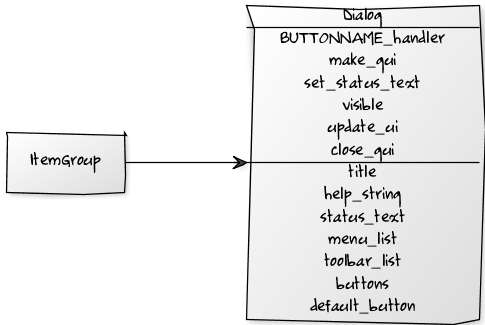
\includegraphics[]{uml-dialog}
  \caption{Standard methods and properties for a dialog.}
  \label{fig:uml-dialog}
\end{figure}


%%%%%%%%%%%%%%%%%%%%%%%%%%%%%%%%%%%%%%%%%%%%%%%%%%
%% Views
\section{Views}
\label{sec:views-1}

View provide a means to customize the look of a dialog or item
group. A view is simply a container. The constructors specify the
child components as either strings indicating items, or other views. A
\args{context} allows the appropriate item to be found from the
string. By default, this context is the calling dialog or item group,
but need not be. This can be useful if the item to display is in
another item group.

\subsection{Types of views}
\label{sec:types-views}

The various views are described by their man pages. They are very
similar to the \pkg{gWidgets} containers except for that provided by
the \constructor{aContext} constructor. This view does not place its items in a
container, but rather provides a means to specify a context. This is
useful if an item comes from another item group, but you wish the
alignment of the item to be as others.

\begin{table}
\centering
\label{tab:view-constructors}
\caption{Table of view constructors.}
\begin{tabular}{@{}lp{0.7\textwidth}@{}}
\toprule

Constructor&Description\\
\midrule
aContainer&Basic container, uses tabular layout\\aTableLayout&Tabular layout with more than 2 columns\\aGroup&Box container to pack in children left to right or top to bottom\\aFrame&Box container with decorative frame\\anExpandGroup&Box container with trigger to hide\\aPanedGroup&Two pane container\\aNotebook&Notebook container\\aContext&Provide context for an item or items
\\ \bottomrule
\end{tabular}
\end{table}

\subsection{Enabled and visible}
\label{sec:enabled-visible}

In a previous example we illustrated the view method
\meth{enabled\_when} which is called whenever a property value is
changed. If this returns \code{FALSE}, then this part of the view has
its sensitivity disabled.

Similarly, there is a \meth{visible\_when} method that can be used to
hide a portion of a GUI until something occurs.


\subsection{Editors}
\label{sec:editors}

A view is used to layout one or more items, whereas each item itself
has its interface produced by an editor. Editors are specified by the
item constructor, with a default editor usually being
appropriate. Some items provide more than one possible editor, for
instance the \constructor{choiceItem}. To specify which editor to use, the
property \property{editor\_style} is set to the name of the different
editor. 

To define a new item, one must also provide an editor or use one of
the existing ones. 




% http://yuml.me/diagram/scruffy/class/
% [View|
% get_widget_by_name; get_widgets; make_ui;is_realized; enabled; visible
% | attr; 
% ]

\begin{figure}
  \centering
  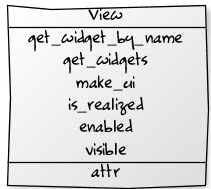
\includegraphics[]{uml-view}
  \caption{Standard methods and properties for a view.}
  \label{fig:uml-view}
\end{figure}

% http://yuml.me/diagram/scruffy/class/
% [View] ->
% [Editor 
% |make_ui; visible; enabled; instance; set_valid; set_invalid
% |editor_style;attr;
% ]

\begin{figure}
  \centering
  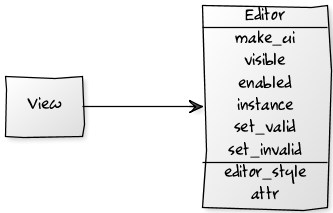
\includegraphics[]{uml-editor}
  \caption{Standard methods and properties for an editor.}
  \label{fig:uml-editor}
\end{figure}


\subsection{Integration with \pkg{gWidgets}}
\label{sec:integr-with-pkggw}

The \pkg{gWidgets} package is used to provide the link between the
\pkg{traitr} objects and a graphical toolkit package, such as
\pkg{RGtk2}. In order to customize the appearance of the editors, one
passes through the \args{attr} argument a list of values for
\pkg{gWidgets} constructors. 

To place a \pkg{traitr} GUI within a \pkg{gWidgets} GUI, one can use
either the \meth{make\_ui} method of an item obect, or the
\meth{make\_gui} method of an itemgroup object, as both have a
\code{container} argument to pass in a \code{gWidgets} container.

To place a \code{gWidgets} object within  a \code{traitr} object is
more difficult, as there is no API for this (yet). At this point, one
can create a container object and place it within that. The container
object has a property \code{container} that stores the \pkg{gWidgets}
container needed. However, this isn't available until after the GUI
has been drawn.

This idea is illustrated below:
\begin{Schunk}
\begin{Sinput}
 dlg <- aDialog(items=list(x=numericItem(1)))
 g <- aGroup()                           # define outside view to access later
 view <- aContainer("x",g)
 dlg$make_gui(gui_layout=view, visible=FALSE) # postpone showing, but create containers
 l <- glabel("Look ma, a gWidgets label", cont = g$container) # how to find container
 dlg$visible(TRUE)
\end{Sinput}
\end{Schunk}

\subsection{Adding elements to an already drawn GUI}
\label{sec:adding-elements-an}

In \pkg{gWidgets}, and indeed only because it is a common feature of
the graphical toolkits, one can add elements to a previously drawn
GUI. In \pkg{gWidgets}, this is done through the \code{add} method of
containers (although this is usually called indirectly in the
containers construction).

However, to add to a GUI using \pkg{traitr} is not so direct. Using
the previous idea though allows it to be done provided you provide a
place where objects will be added in the GUI construction. This is
implemented by hiding the visibility of the container through its
\meth{visible\_when} method.

\begin{Schunk}
\begin{Sinput}
 dlg <- aDialog(items=list(x=numericItem(0)))
 g <- aGroup(visible_when=function(.) FALSE) # suppress showing
 view <- aContainer("x", g)
 dlg$make_gui(gui_layout=view)
 ## now to add to the GUI at g:
 ig <- anItemGroup(list(y=stringItem("a string")))
 ig$make_gui(container=g)
 g$visible_when <- function(.) TRUE
 dlg$update_ui()                        
\end{Sinput}
\end{Schunk}
The call to the \meth{update\_ui} method is also done whenever a
value changes, but in this case we want it to be done immediately so
the string item shows up.


\section{Some examples}
\label{sec:some-examples}
Some additional examples follow that are a bit more involved.


\subsection{chooseCRANmirror}
\label{sec:choosecranmirror}

The function \code{chooseCRANmirror} provides a GUI for selecting a
CRAN mirror, providing a table to choose the mirror from and a button
to click once the selction is done. Here we give a slightly better
alternative, with a bit more information and also connect to a double
click event. The
key function, \code{setCran}, is taken from the original with slight modification.
\begin{Schunk}
\begin{Sinput}
 m <- getCRANmirrors(all = FALSE, local.only = FALSE)[,c(1,2,4)]
 setCran <- function(.,...) {
   URL <- .$get_cran()
   repos <- getOption("repos")
   repos["CRAN"] <- gsub("/$", "", URL[1L])
   options(repos = repos)
   .$close_gui()
 }
\end{Sinput}
\end{Schunk}
Now we define our model, and use the default view.
\begin{Schunk}
\begin{Sinput}
 dlg <- aDialog(items=list(
                  cran=choiceItem(value=NA, values=m,
                    show_label=FALSE,  # suppress label
                      attr=list(chosencol=3, size=c(400,500)) #chosencol is URL one, not first
                    )
                  ),
                title="Choose a CRAN Mirror",
                help_string="Click a mirror, then OK, or double click on mirror",
                OK_handler=setCran,                 # OK button click
                property_cran_value_changed=setCran # double click
                )
 dlg$make_gui()
\end{Sinput}
\end{Schunk}


\subsection{The tkdensity dialog}
\label{sec:tkdensity-dialog}

\begin{figure}
  \centering
  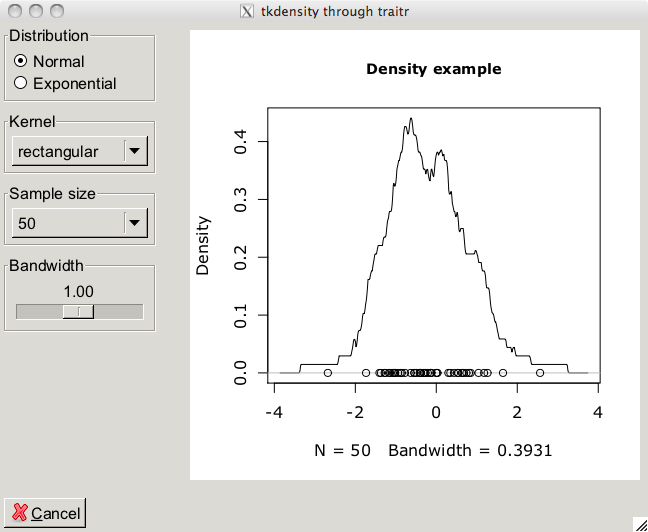
\includegraphics[width=.6\textwidth]{tkdensity-traitr}
  \caption{A dialog similar to that of the tkdensity demo in the
    \pkg{tcltk} package.}
  \label{fig:tkdensity-traitr}
\end{figure}


The \code{tkdensity} demo is a standard in the \pkg{tcltk}
package. Here we redo the demo using \pkg{traitr}
(Figure~\ref{fig:tkdensity-traitr}). This function will make the
density plot for us, in a manner similar to that of the demo.
\begin{Schunk}
\begin{Sinput}
   replot <- function(.) {
     l <- .$to_R()
     f <- function(dist, kernel, n, bw,...) {
       y <- switch(dist, "Normal"=rnorm(n), rexp(n))
       plot(density(y,  bw=bw, kernel=kernel), xlim=range(y)+c(-2,2), main="Density example")
       points(y, rep(0,n))
     }
     do.call(f,l)
   }
\end{Sinput}
\end{Schunk}
Here we define the items and the dialog properties. There are 5 main
items, including the graphic device. The labels are suppressed, as we
use a frame to set off similar to the original example. 
\begin{Schunk}
\begin{Sinput}
 dlg <- aDialog(items=list(
                  dist=choiceItem("Normal", values=c("Normal","Exponential"),
                    show_label=FALSE),
                  kernel=choiceItem("gaussian",
                    values=c("gaussian", "epanechnikov", "rectangular",
                      "triangular", "cosine"),
                    show_label=FALSE),
                  n=choiceItem(50L, as.integer(c(50,100,200,300)),
                    show_label=FALSE),
                  bw=rangeItem(value=1, from=0.05, to=2.00, by=0.05,
                    show_label=FALSE),
                  out=graphicDeviceItem()
                  ),
                help_string="Adjust a parameter to update graphic",
                title="tkdensity through traitr",
                buttons="Cancel",
                model_value_changed=replot)
\end{Sinput}
\end{Schunk}
Our layout places the controls on the left within frames, and the
graphic device on the right. We use only the 'Cancel' button to match,
somewhat, the demo.
\begin{Schunk}
\begin{Sinput}
 view <- aGroup(aContainer(aFrame("dist", label="Distribution"),
                           aFrame("kernel", label="Kernel"),
                           aFrame("n", label="Sample size"),
                           aFrame("bw", label="Bandwidth")
                           ),
                "out",
                horizontal=TRUE)
 dlg$make_gui(gui_layout=view)
 replot(dlg)                           # initial plot
\end{Sinput}
\end{Schunk}

\subsection{The \code{itemList} item}
\label{sec:codeitemlist-item}

One of the drawbacks with this framework is that it is not geared
around \R's vectorized treatment of parameters and data. Although, the
basic items, such as \code{numericItem}, can hold a vector of data,
the editor for that is not helpful. The \code{itemList} item is used
to get around this. It stores a list of items or itemgroups and has a
means to edit on a per item basis. The basic usage depends on
specifying how new items are to be constructed. The argument
\code{item\_factory} is where this is specified. Here are a few
examples of it being used.

The most basic usage is to edit a vector of values, as here where the
items are numeric.
\begin{Schunk}
\begin{Sinput}
 i1 <- itemList(items=list(),
                items_names="x",
                item_factory=function(.) numericItem(0)
                )
 i1$make_ui(container=gwindow("Basic Use"))
\end{Sinput}
\begin{Soutput}
NULL
\end{Soutput}
\end{Schunk}
If we add some items, we see that the \code{to\_R} method will return
a list of item values.
\begin{Schunk}
\begin{Sinput}
 ## add some items offline
 for(i in 1:2) i1$append_item(i1$item_factory())
\end{Sinput}
\end{Schunk}
\begin{Schunk}
\begin{Sinput}
 i1$to_R()
\end{Sinput}
\begin{Soutput}
$Anonymous
$Anonymous$Anonymous
[1] 0

$Anonymous$Anonymous
[1] 0
\end{Soutput}
\end{Schunk}

If we want to make a data frame editor, we can do so as
follows. Rather than have a single item, we have an item group to
edit. The new \code{to\_string} method is needed as this method gets
called to label the table that shows the list of defined items. It
should return a character vector of length $1$.
\begin{Schunk}
\begin{Sinput}
 i2 <- itemList(items=list(),
                items_names="Data frame rows",
                item_factory=function(.) {
                  ig <- anItemGroup(items=list(a=numericItem(0), b=stringItem("")))
                  ig$to_string <- function(.) .$get_b()
                  ig
                })
\end{Sinput}
\end{Schunk}

We provide a custom \code{to\_R} method to take the output and
place into a data frame. (Suggestions for a more elegant solution here
are most welcome.)
\begin{Schunk}
\begin{Sinput}
 i2$to_R <- function(.) {
   items <- .$get_value()
   if(length(items) == 0) {
     out <- as.data.frame(.$item_factory()$to_R(), stringsAsFactors=FALSE)[0,]
   } else {
     out <- as.data.frame(items[[1]]$to_R(), stringsAsFactors=FALSE)
     if(length(items) > 1) {
       for(i in 2:length(items))
         out[i,] <- items[[i]]$to_R()
     }
   }
   out
 }
\end{Sinput}
\end{Schunk}

And the basic call:
\begin{Schunk}
\begin{Sinput}
 i2$make_ui(container=gwindow("Basic Use to make data frame"))
\end{Sinput}
\begin{Soutput}
NULL
\end{Soutput}
\end{Schunk}

Finally, the manual page's example illustrates the \code{post\_process}
method call and how to add in icons to the item list.


\subsection{A GUI for read.csv and read.table}
\label{sec:gui-read.csv-read.t}



\begin{figure}
  \centering
  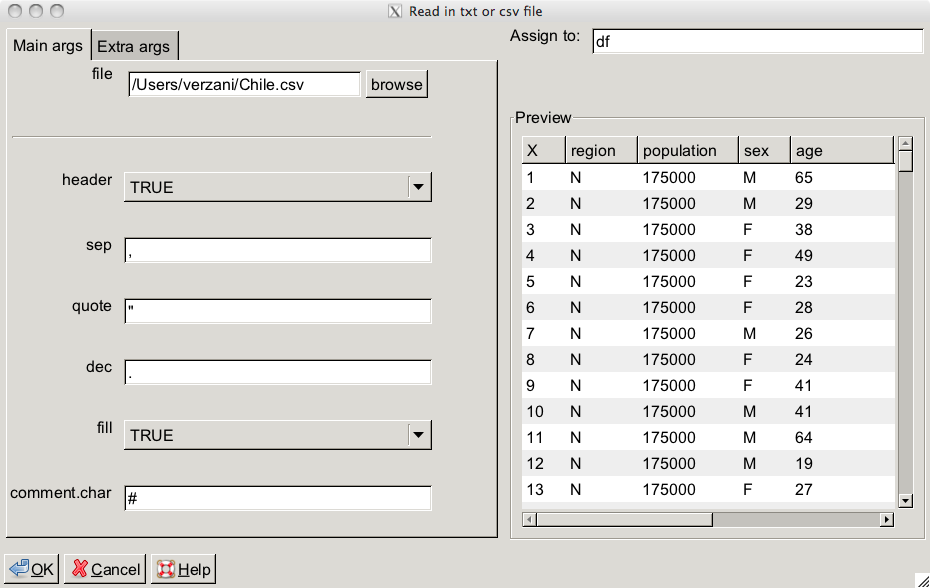
\includegraphics[width=.6\textwidth]{read-csv-gui}
  \caption{A GUI for the \code{read.csv} and \code{read.table} functions.}
  \label{fig:read-csv-gui}
\end{figure}

This example shows how the mapping between argument and \pkg{traitr}
items proceeds in a straightforward manner. We provide a GUI
(Figure~\ref{fig:read-csv-gui}) for
\code{read.csv} and \code{read.table}. While these both work quite
easily with the default arguments, in the case they don't the
arguments can be numerous. This GUI allows one to specify the
arguments (except for typing in names and class types, although that
could have been implemented using \constructor{stringItem}s which
evaluate their argument first.

First, the model part:
\begin{Schunk}
\begin{Sinput}
 dlg <- aDialog(items=list(
                  file=fileItem("", attr=list(
                                      filter=list("CSV or TXT"=list(
                                                    patterns=c("*.csv","*.txt")
                                                    ),
                                        "All files" = list(patterns=c("*"))
                                        ))),
                  header=trueFalseItem(TRUE, tooltip=paste("Variable onfirst line?")),
                  sep=stringItem("", tooltip="Field separator character"),
                  quote=stringItem("", tooltip="Set of quoting characters"),
                  dec=stringItem(".", tooltip="Character used for decimal points"),
                  as.is=trueFalseItem(!default.stringsAsFactors(), 
                    tooltip="Do not convert character to factor"),
                  na.strings=stringItem("NA", tooltip="Strings to be NA", eval=TRUE),
                  nrows=integerItem(-1, tooltip="Max number of rows to read"),
                  skip=integerItem(0, tooltip="Number of lines to skip at header"),
                  check.names=trueFalseItem(TRUE, tooltip="If TRUE ensure names are valid"),
                  fill=trueFalseItem(TRUE, tooltip="Fill unequal length rows if TRUE"),
                  strip.white=trueFalseItem(TRUE),
                  blank.lines.skip=trueFalseItem(TRUE, tooltip="If TRUE, skip blank lines"),
                  comment.char=stringItem("#", tooltip="Comment character"),
                  allowEscapes=trueFalseItem(TRUE, tooltip="C-style escapes read verbatim?"),
                  stringsAsFactors=trueFalseItem(default.stringsAsFactors(), 
                    tooltip="Characters converted to factors"),
                  fileEncoding=stringItem(""),
                  encoding=stringItem("unknown"),
                  ## our things
                  assign.to=stringItem("df", label="Assign to:"),
                  output=tableItem(attr=list(size=c(400,400)), show_label=FALSE),
                  file.type=stringItem("")
                  ),
                title="Read in txt or csv file",
                help_string="Select a file, then adjust parameters."
                )
\end{Sinput}
\end{Schunk}
The \code{file} object has \pkg{gWidgets} arguments passed through to
filter which files are displayed. Otherwise, this is a straightforward
mapping of arguments to type. The last three are there for the GUIs usage.

The view separates out the main arguments from some secondary ones,
using the notebook container; and provides a place for the assignment
and preview features. Above, we manually set the size in the \code{output}
object above, as
it does not gracefully allocate enough size to itself when the
\pkg{gWidgetsRGtk2} backend is used.
\begin{Schunk}
\begin{Sinput}
 view <- aGroup(aNotebook(
                          aNotebookPage("file",
                                        separatorItem(),
                                        "header", "sep","quote",
                                        "dec", "fill", "comment.char",
                                        label="Main args"),
                          aNotebookPage("as.is","na.strings","nrows","skip",
                                        "check.names","fill","strip.white","blank.lines.skip",
                                        "allowEscapes","stringsAsFactors",
                                        separatorItem(),
                                        "fileEncoding", "encoding",
                                        label="Extra args")
                          ),
                aContainer("assign.to",
                           aFrame("output", label="Preview")
                           ), 
                horizontal=TRUE)
\end{Sinput}
\end{Schunk}

The main function called to update the UI is this one, which 
checks the file type, then reads in the file using either
\code{read.csv} or \code{read.table}. If successful, it returns the
data frame.
\begin{Schunk}
\begin{Sinput}
 dlg$read_file <- function(., file.type, output, assign.to, ...) {
   if(file.type != "") {
     out <- try(do.call(sprintf("read.%s",file.type), list(...)), silent=TRUE)
     if(inherits(out, "try-error")) {
       cat("Error reading file of type,", file.type, "\n")
       out <- data.frame(V1="")
     }
   } else {
     out <- data.frame(V1="")
   }
   return(out)
 }
\end{Sinput}
\end{Schunk}

To integrate the \code{read\_file} method, we set up the following
handler for control:

\begin{Schunk}
\begin{Sinput}
 dlg$model_value_changed <- function(.) {
   fname <- .$get_file()
   if(file.exists(fname)) {
     for(i in c("txt","csv")) {
       if(grepl(paste("\\.",i,sep=""), fname))
         .$set_file.type(c(txt="table",csv="csv")[i])
     }
   }
   switch(.$get_file.type(),
          "csv"={.$set_sep(","); .$set_quote('\"')},
          "table"={},
          {}
          )
   .$set_output(.$do_call("read_file",.$to_R()))
 }
\end{Sinput}
\end{Schunk}

This method sets up a call to our \meth{read\_file} using the values
found from the \meth{to\_R} method. The use of \meth{do\_call} is
identical to the familiar \code{do.call} function, except it
gracefully handles the instance where the method does not exist.

This method is called whenever a model value is changed, even the
\code{output} value, say, which is not really necessary. If this
inefficiency bothers you, a different manner is presented at the end.

Finally, we change the default \meth{OK\_handler} to output the
value to the given name. We use a \pkg{gWidgets} call to
\constructor{gconfirm} to avoid overwriting a variable name without permission.

\begin{Schunk}
\begin{Sinput}
 dlg$OK_handler <- function(.) {
   out <- .$do_call("read_file",.$to_R())
   assign.to <- .$get_assign.to()
   if(exists(assign.to, envir=.GlobalEnv)) {
     if(!gconfirm(sprintf("Overwrite variable %s?", assign.to)))
       return()
   }
   assign(assign.to, out, envir=.GlobalEnv)
 }
\end{Sinput}
\end{Schunk}

The GUI is drawn as usual now:
\begin{Schunk}
\begin{Sinput}
 dlg$make_gui(gui_layout=view)
\end{Sinput}
\end{Schunk}

%% Still slow, but much faster with different calls to set_XXX,
%% get_XXX in ItemGroup
% This GUI shows a limitation of the framework -- it is a bit slow. The
% updating of the preview when the file changes takes a longer than
% expected amount of time. It is hoped that careful profiling can bring
% this down.

To see one way to get the dialog to update only in response to the
appropriate changing of the model, we could replace the
\meth{model\_value\_changed} code with the following. First we
have a different response when the file is changed, as we need to find
the file type and adjust some arguments for CSV files.
\begin{Schunk}
\begin{Sinput}
 dlg$property_file_value_changed <- function(., value, old_value) {
   if(file.exists(value)) {
     for(i in c("txt","csv")) {
       if(grepl(paste("\\.",i,sep=""), value))
         .$set_file.type(c(txt="table",csv="csv")[i])
     }
   }
   switch(.$get_file.type(),
          "csv"={.$set_sep(","); .$set_quote('\"')},
          "table"={.$set_output(.$do_call("read_file",.$to_R()))},
          {}
          )
 
 }
\end{Sinput}
\end{Schunk}

The call to \meth{set\_output} will be done by both \meth{set\_sep} and
\meth{set\_quote} as well, so we don't repeat more than we have to.

Now to update the preview when an argument is changed, we set up the
appropriate \code{property\_XXX\_value\_changed} methods, as follows:
\begin{Schunk}
\begin{Sinput}
 nms <- names(dlg$get_items())
 nms <- setdiff(nms, c("file","file.type","assign.to","output"))
 QT <- sapply(nms, function(i) {
   assign(sprintf("property_%s_value_changed",i),
          function(., ...) {
            .$set_output(.$do_call("read_file",.$to_R()))
          },
          envir=dlg)
 })
\end{Sinput}
\end{Schunk}
The assignment of the method within the environment takes advantage of
\pkg{proto} objects being environments.

\subsection{A view data frame by row GUI}
\label{sec:view-data-frame}

\begin{figure}
  \centering
  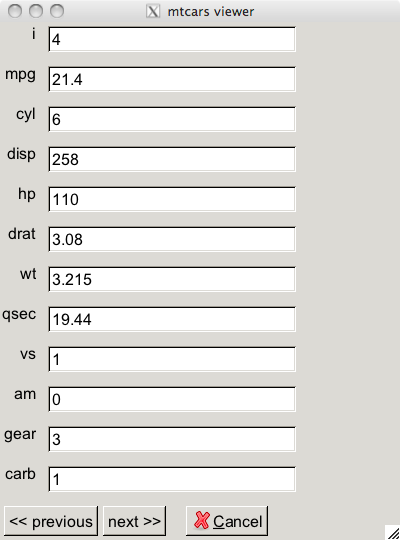
\includegraphics[width=.6\textwidth]{df-scroll}
  \caption{A GUI to scroll through the rows of a data frame.}
  \label{fig:df-scroll}
\end{figure}

A common GUI for viewing data on web sites basically shows each row of
a data frame as editable data. In statistics terms, we scroll through
the cases in a data set.  Below, we leave the editable part as an
exercise, but show how the method \meth{set\_model} can be used to
effect this type of GUI.

This function creates a list of items from a row in the data
frame. The \meth{set\_model} method for a dialog takes a dialog or
item group for an argument. The output of this function will provide
the items value.
\begin{Schunk}
\begin{Sinput}
 m <- mtcars
 nms <- names(m)
 make_model <- function(i) {
   l <- list(i = integerItem(i))
   for(j in 1:ncol(m)) {
     l[[nms[j]]] <- numericItem(m[i,j])
   }
   l
 }
\end{Sinput}
\end{Schunk}
Here we initialize the dialog and make two buttons to scroll through
the rows. The \code{set\_row} method finds the next row to show, then
creates an item group which is used for our new model. The same
extractor method, \code{get\_i} is used in the button handlers.
\begin{Schunk}
\begin{Sinput}
 dlg <- aDialog(items=make_model(1),
                title="Data frame scroller",
                help_string="Press buttons to scroll through data set",
                buttons=c("<< previous","next >>","SPACE","Cancel"),
                set_row=function(.,i) {
                  if(i < 1)
                    i <- nrow(m)
                  if(i > nrow(m))
                    i <- 1
                  ig <- make_model(as.numeric(i))
                  .$set_model(anItemGroup(items=ig))
                },
                previous_handler=function(.) {
                  i <- as.integer(.$get_i())
                  .$set_row(i-1)
                },
                next_handler=function(.) {
                  i <- .$to_R()$i        # same but different
                  .$set_row(i + 1)
                })
\end{Sinput}
\end{Schunk}
We now make the GUI (Figure~\ref{fig:df-scroll}).
\begin{Schunk}
\begin{Sinput}
 dlg$make_gui()
\end{Sinput}
\end{Schunk}
That's it. We leave for later perhaps using a scroller to scroll
through the rows, or a means to edit the values and store in the data frame.

\subsection{A Wizard GUI}
\label{sec:wizard-gui}


A wizard, or multi-page dialog is a common GUI arrangement. Here is
one way to implement such a feature, maybe not the best. We create a
model to store our values and use instances of this model and views
to show just part.
\begin{Schunk}
\begin{Sinput}
 model <- aDialog(items=list(
                    a=stringItem(""),
                    b=stringItem("")
                  )
                  )
 dlg1 <- aDialog(buttons="Next",
                 Next_handler=function(.) {
                   dlg2$make_gui(gui_layout=view2)
                   .$close_gui()
                 })
 view1 <- aContainer("a", context=model)
 dlg2 <- aDialog(buttons = c("Finished"),
                 Finished_handler = function(.) {
                   print(model$to_R())
                   .$close_gui()
                 })
 view2 <- aContainer("b", context=model)
 dlg1$make_gui(gui_layout=view1)
\end{Sinput}
\end{Schunk}
                 
\subsection{A "spotfire" like demo}
\label{sec:spotfire-like-demo}

\begin{figure}
  \centering
  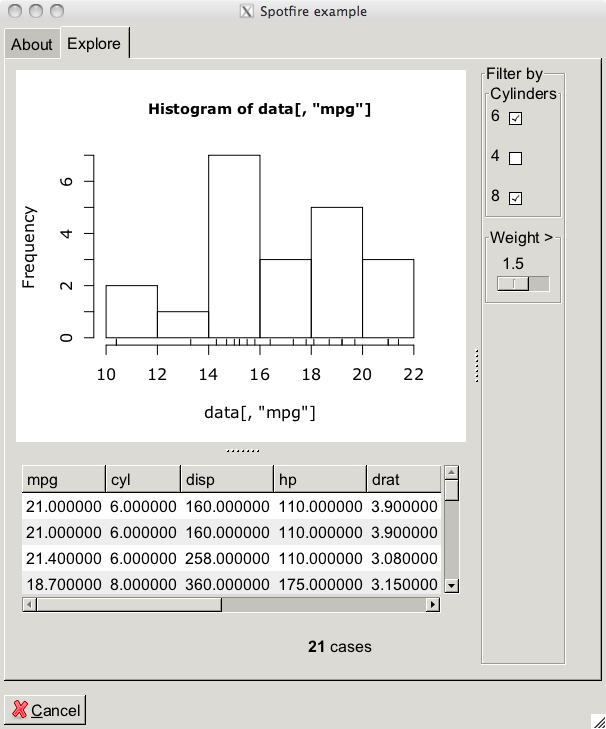
\includegraphics[width=0.6\textwidth]{spotfire}
  \caption{A GUI designed around the graphical summary of a data frame with controls to narrow the values displayed. }
  \label{fig:spotfire}
\end{figure}


The purveyor of S-Plus has a product to create interactive web pages
from within S-Plus. See \url{http://spotfire.tibco.com} for
details. The examples shown are of a similar type. A GUI is
constructed around a specific data set and has some graphic to
summarize the data and some filter controls to filter the display of
the data. Additionally, there is some interactivity between the
graphic and the data table. The latter we don't illustrate below, but
we do illustrate how to use \pkg{traitr} to make a similar type of
GUI. 

This example will also demonstrate how one can create components with
\pkg{traitr} to be used within other parts of a GUI.

The Spotfire demos all have a description page. Here illustrate how
PANGO markup can be used with a label item to provide some markup for
the instructions.
\begin{Schunk}
\begin{Sinput}
 theDesc <- paste("<b>Spotfire</b>",
                  "The Spotfire web player (http://spotfire.tibco.com)",
                  "has several demos built around a somewhat similar set-up:",
                  "a description page, a data set, a graphic display of the data, and a set",
                  "of controls to filter out the data that is being displayed in the graphic.",
                  "",
                  "This example shows how <b>traitr</b> can be used to make a simple version of such.",
                  "",
                  "Click the <i>Explore</i> tab to begin.",
                  sep="\n")
\end{Sinput}
\end{Schunk}
The data set we will use here is the standy \code{mtcars} one. This
would be customized to the GUI in question. Our table display will
also include a label to display the number of selected cases (rows)
after filtering has occurred.
\begin{Schunk}
\begin{Sinput}
 theData <- mtcars
 makeLabel <- function(nr) sprintf("<b>%s</b> cases",nr)
 dataDisplay <- anItemGroup(items=list(
                              data = tableItem(theData, name="data", attr=c(expand=TRUE)),
                              label = labelItem(makeLabel(nrow(theData)), attr=c(markup=TRUE, expand=FALSE))
                              ),
                            attr=c(expand=TRUE)
                            )
\end{Sinput}
\end{Schunk}
We define this handler to synchronize the label with the size of the
data being displayed.
\begin{Schunk}
\begin{Sinput}
 ## synchronize labe with data dimension
 dataDisplay$property_data_value_changed <- function(., value, old_value)
   .$set_label(makeLabel(nrow(.$get_data())))
\end{Sinput}
\end{Schunk}

We wish to specify the layout for the data table here, rather than in
a monolithic specification when the entire GUI is constructed. By
doing so, we could reuse this in other GUIs without much fuss. To do
so, we redefine the method to define the default layout.
\begin{Schunk}
\begin{Sinput}
 dataDisplay$make_default_gui_layout <- function(.) {
   aGroup("data",
          aGroup(labelItem("", attr=c(expand=TRUE)),"label", horizontal=TRUE),
          horizontal=FALSE)
 }
\end{Sinput}
\end{Schunk}


Our filter controls are chosen to illustrate how we could use a slider
or a checkbox to narrow the number of cases displayed.  

We begin with a filter to narrow down by levels of a variable. The
\code{get\_selected} method returns a logical vector of the cases that
are selected.  For this, we also specify a default layout. Together,
this creates a component that can easily be incorporated into another
item group.
\begin{Schunk}
\begin{Sinput}
 var <- "cyl"
 varLevels <- sort(unique(theData[, var]))
 cylFilter <- anItemGroup(name=var,
                          items=list(
                            choice=choiceItem(varLevels, varLevels,
                              by_index=FALSE, multiple=TRUE, show_label=FALSE)
                            ),
                          data=theData[, var],
                          get_selected = function(.) {
                            choice <- .$get_item_by_name("choice")
                            value <- choice$get_choice()
                            values <- choice$get_values()
                            vals <- values[values %in% value]
                            .$data %in% vals
                          },
                          make_default_gui_layout=function(.) {
                            aFrame("choice", label="Cylinders")
                         })
\end{Sinput}
\end{Schunk}

This shows a filter for a numeric variable.
\begin{Schunk}
\begin{Sinput}
 var1 <- "wt"
 rng <- range(theData[, var1])
 wtFilter <- anItemGroup(name=var1,
                         items=list(
                           weight=rangeItem(value=rng[1] - .2, from=rng[1], to=rng[2], by=.2,
                             show_label=FALSE, label="Weight >")
                           ),
                         data=theData[,var1],
                         get_selected=function(.) {
                           .$data >= .$to_R()$weight
                         },
                         make_default_gui_layout=function(.) {
                           aFrame("weight", label="Weight > ")
                         }
                         )
\end{Sinput}
\end{Schunk}

Our \code{filters} item group will hold the two. Here we specify the
layout using a frame.
\begin{Schunk}
\begin{Sinput}
 filters <- anItemGroup(items=list(cylFilter, wtFilter))
 filters$make_default_gui_layout <- function(.) {
   aFrame(var,
          var1,
          label="Filter by",
          attr=c(size=c(300,-1)))
 }
\end{Sinput}
\end{Schunk}

Our main method is called when a filter value is changed. It computes
the indices of the cases that are still valid. This task is made
simpler by defining the \code{get\_selected} methods, as these return
the logical values we wish. 

\begin{Schunk}
\begin{Sinput}
 filters$model_value_changed <- function(.) {
   items <- .$get_items()
   ind <- as.logical(items[[1]]$get_selected() * items[[2]]$get_selected())
   dlg$update_data(ind)
 }
\end{Sinput}
\end{Schunk}



With the pieces above, creating the main GUI is now
straightforward. The items are four in number: the label, the data,
the graphic device and the filter area.
\begin{Schunk}
\begin{Sinput}
 dlg <- aDialog(items=list(
                  Description=labelItem(theDesc, attr=c(markup=TRUE)),
                  gd = graphicDeviceItem(),
                  filters,
                  dataDisplay
                  ),
                title="Spotfire example",
                buttons="Cancel"
                )
\end{Sinput}
\end{Schunk}
When the data is changed, we want the graphic to be updated.
\begin{Schunk}
\begin{Sinput}
 dlg$property_data_value_changed <- function(., value, old_value) 
   .$draw_graphic()
\end{Sinput}
\end{Schunk}
This method was referred to above in the method calls for
filtering. The filter updates the data, and then the above method is
called to update the graphic.
\begin{Schunk}
\begin{Sinput}
 dlg$update_data <- function(., index) {
   if(missing(index))
     data <- theData
   else
     data <- theData[index,]
   dataDisplay$set_data(data)
 }
\end{Sinput}
\end{Schunk}

Finally, we make the drawing of the graphic a separate method, so we
can call it without having to update the data set. We don't work very
hard in the graphical summary of data.
\begin{Schunk}
\begin{Sinput}
 dlg$draw_graphic <- function(.) {
   data <- dataDisplay$get_data()
   if(nrow(data)) {
     hist(data[,"mpg"])
     rug(data[, "mpg"])
   } else {
     plot.new()
   }
 }
\end{Sinput}
\end{Schunk}

Finally, we use paned groups to layout our GUI, allowing the user to
give more area to the data table if desired.

\begin{Schunk}
\begin{Sinput}
 ## Layout for main GUI
 lyt <- aNotebook(aNotebookPage("Description",
                                label="About"
                                ),
                  aNotebookPage(aPanedGroup(
                                            aPanedGroup("gd",
                                                        dataDisplay,
                                                        horizontal=FALSE),
                                            filters),
                                label="Explore"
                                )
                  )
\end{Sinput}
\end{Schunk}

Since the GUI takes a few seconds to load, we first call the
\code{loadingAnimation} window to give the user some feedback.
\begin{Schunk}
\begin{Sinput}
 w <- loadingAnimation()
 dlg$make_gui(gui_layout=lyt)
 w$close()
\end{Sinput}
\end{Schunk}
\end{document}



